\section{INTRODUÇÃO}

Água é indiscutivelmente o fator isolado mais importante, com possível
exceção para luz solar e o ar que não têm disponibilidade limitada,
para o desenvolvimento das plantas \cite{Chesworth2007}.  A água
presente no solo desempenha inumeráveis funções de ordem química,
física e biológica como, por exemplo, dissolver e transportar
nutrientes para as plantas além de também ser considerada um nutriente
\cite{Brady2009}.  O excesso de água no solo pode diminuir ou impedir
o desenvolvimento das plantas devido a uma reduzida aeração, enquanto
deficiências podem causar estresse hídrico e, se severa o suficiente,
o murchamento e morte da planta. Para uma produção eficiente, um
fornecimento constante de água é necessário durante o ciclo da planta
para atender as necessidades hídricas e promover a dissolução,
transporte e absorção de nutrientes. O conteúdo de água também
influencia a qualidade de operações de manejo do solo e colheita.

\newpage
\section{RETENÇÃO DE ÁGUA E TAMANHO DE POROS}\label{sc-craporos}

Dada a relação que existe entre tamanho de poros e tensão matricial
é possível chegar à distribuição de frequência
de tamanho de poros quando o modelo \citeonline{VanGenuchten1980} é
usado para representar a CRA \cite{Reynolds2002a}. Essa relação não
pode ser considerada isoladamente pois fatores que alteram as
propriedades da água de um solo para o outro a modificam, como a
concentração de íons e a temperatura. Por outro lado, fixadas as
demais variáveis, essa relação permite explorar a conexão existente
entre a retenção de água e distribuição de tamanho de poros. Além do
mais, a partir dessa relação, é possível verificar que o parâmetro $S$
proposto por \citeonline{Dexter2004} é o parâmetro de escala que
representa o grau de dispersão de valores ao redor do tamanho modal de
poros.

\newpage
\section{MATERIAL E MÉTODOS}\label{sc-methods}

Os dados considerados são medidas de conteúdo de água do solo (m$^3$
m$^{-3}$) em função do potencial matricial (kPa) coletados em campo
sob cultura do cafeeiro no qual se utilizam métodos conservacionistas
e de manejo intensivo do solo \cite{Serafim2011}. Amostras de solo
indeformadas foram coletadas de um solo classificado como Latossolo
Vermelho distroférrico (LVd) em uma lavoura com 3,5 anos de
implantação.

\begin{figure}[!ht]
 \begin{center}
 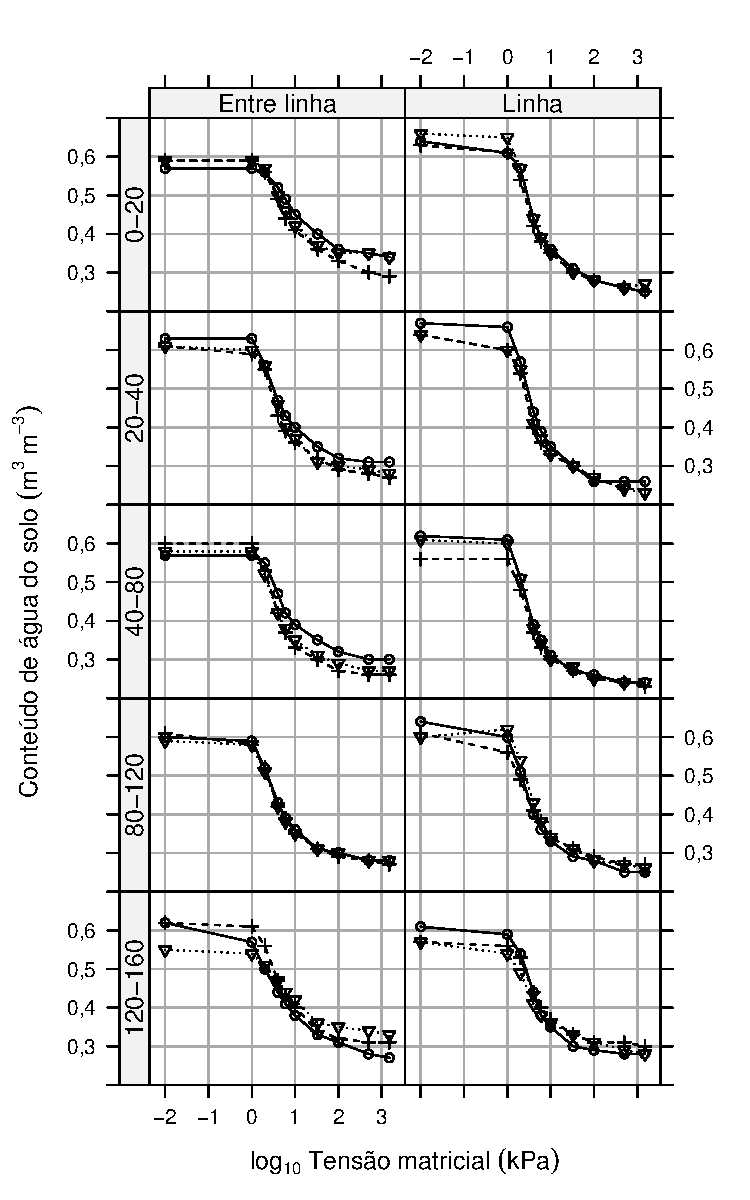
\includegraphics[width=0.7\textwidth]{../figuras/cra_perfil.pdf}
\end{center}
 \caption{Conteúdo de água do solo (m$^3$ m$^{-3}$) em função do
   log$_{10}$ da tensão matricial (kPa) organizado pelas combinações
   entre posição (nas colunas) e profundidade de coleta (nas linhas).
   As três unidades experimentais em cada combinação foram
   identificadas pelos tipos de pontos e linhas}
 \label{fg-craperfil}
\end{figure}

\newpage
\section{RESULTADOS E DISCUSSÃO}\label{sc-results}

Estimativas dos parâmetros foram obtidas para as 30 unidades
experimentais sob as duas parametrizações do modelo van Genuchten.  Os
valores de R$^2$ apontaram boa medida de ajuste pois ficaram entre
98,96\% e 99,88\%.  Pelas estimativas intervalares, considerando os
seis parâmetros definidos pelas duas parametrizações, $U_s$, $U_r$,
$a$, $n$, $S$ e $I$, observamos variação entre unidades experimentais
dentro de uma mesma cela experimental (combinação de posição e
profundidade), entre níveis de profundidade e entre posições de
amostragem (Figura \ref{fg-ICpar}).  Verifica-se que os parâmetros
$U_r$ e $n$, por serem comuns as duas parametrizações, tiveram mesmas
estimativas intervalares independentemente da parametrização.

\begin{figure}[H]
 \begin{center}
 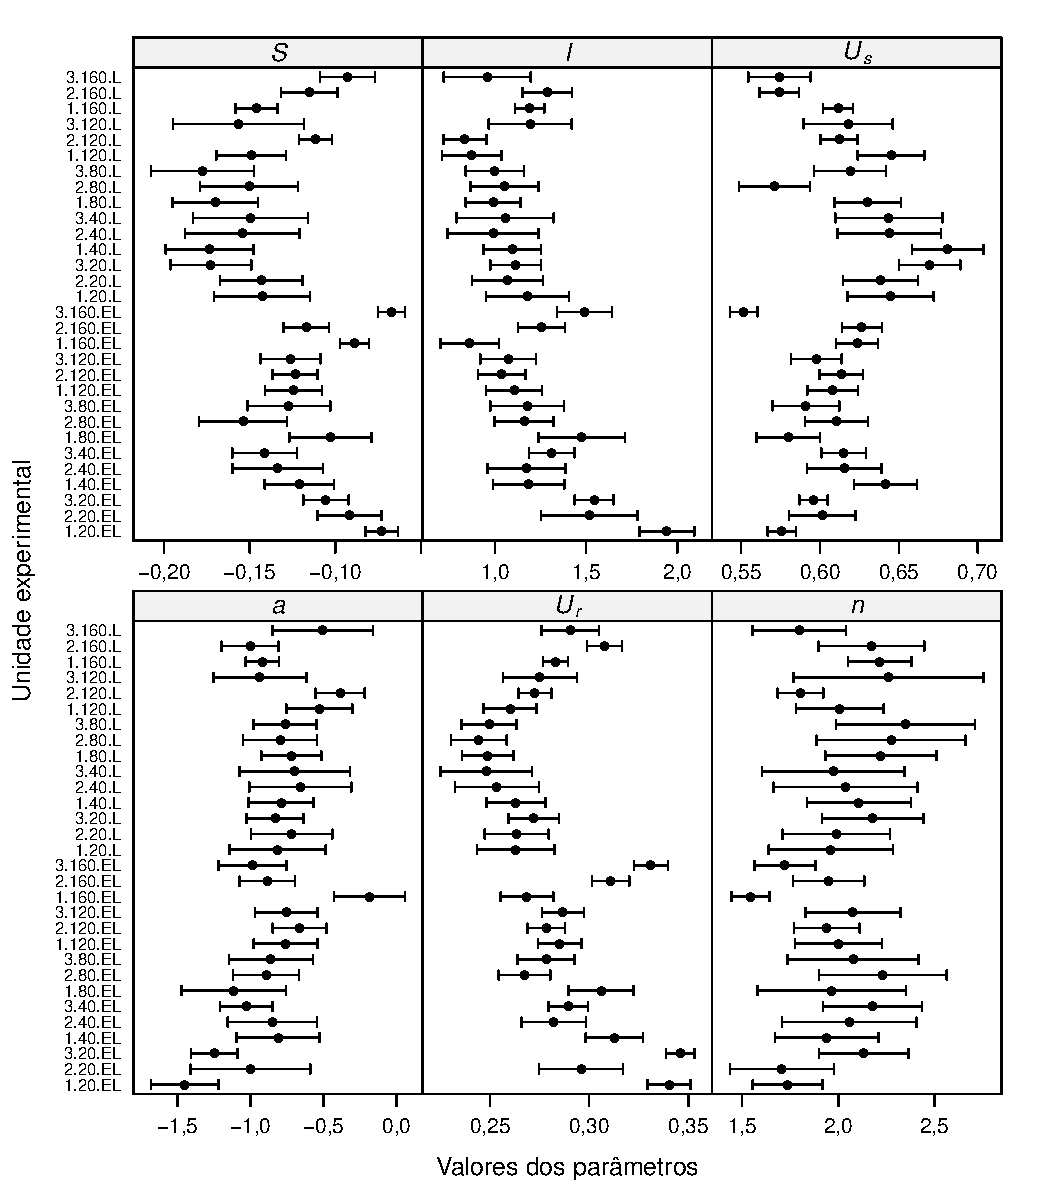
\includegraphics[width=0.8\textwidth]{../figuras/param_ic.pdf}
\end{center}
 \caption{Estimativas intervalares (95\%) pelo método de Wald para os
   parâmetros da CRA considerando as duas parametrizações do modelo
   van Genuchten.  Os rótulos no eixo das coordenadas representam o
   índice da repetição, o nível de profundidade e o nível de posição,
   separados por ponto}
 \label{fg-ICpar}
\end{figure}

\newpage
\section{CONCLUSÕES}\label{sc-conclusion}

Conclui-se que o modelo não linear de efeitos mistos é um método de
análise mais adequado para representar os dados uma vez que toda
informação está contida em um único modelo que permite acomodar os
efeitos de termos fixos e aleatórios, comparar modelos e fazer
predições para a CRA.

\newpage
\addcontentsline{toc}{section}{\hspace*{\distnumber}REFERÊNCIAS}
\begin{center}
\section*{REFERÊNCIAS} 
\end{center}
